\documentclass{article}

\usepackage{tikz}

\begin{document}
    \begin{center}
        
        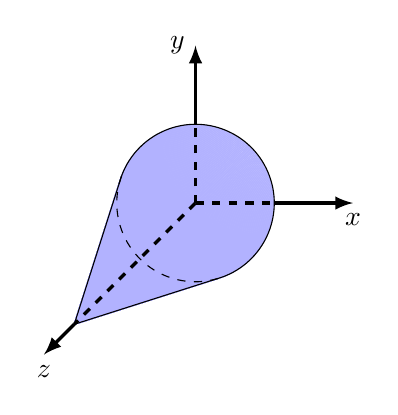
\begin{tikzpicture}
            \coordinate (O) at (0,0,0);

            \foreach \angle in {0, ..., 360}{
                \draw[blue!30, rotate around z=\angle] (1,0,0) -- (0,0,4) -- (-1,0,0);
            }

            \def\angleMin{-70}
            \def\angleMax{160}
            \draw (\angleMin:1cm) arc [start angle=\angleMin, end angle=\angleMax, radius=1cm];
            \draw[dashed] (\angleMax:1cm) arc [start angle=\angleMax, end angle=360+\angleMin, radius=1cm];

            \draw (\angleMin:1cm) -- (0,0,4) -- (\angleMax:1cm);

            \draw[very thick, dashed] (O) -- (1,0,0);
            \draw[very thick, ->, >=latex] (1,0,0) -- (2,0,0) node[below]{\(x\)};
            \draw[very thick, dashed] (O) -- (0,1,0);
            \draw[very thick, ->, >=latex] (0,1,0) -- (0,2,0) node[left]{\(y\)};
            \draw[very thick, dashed] (O) -- (0,0,4) ;
            \draw[very thick, ->, >=latex] (0,0,4) -- (0,0,5) node[below]{\(z\)};
            
        \end{tikzpicture}
    \end{center}
\end{document}